\documentclass[a4paper,12pt]{extarticle}
\usepackage[margin=1.5cm]{geometry}
\usepackage{amsmath, amssymb}
\usepackage{array}
\usepackage{multicol}
\usepackage{helvet}
\usepackage{multirow}
\usepackage{graphicx}
\renewcommand{\baselinestretch}{2}
\renewcommand{\familydefault}{\sfdefault}

\begin{document}


    \begin{tabular}{| c | c | c | c |}
        \hline
        & MATEMÁTICAS & 27/02/2026 & calificación \\
        \hline 

        \multirow{2}{*}{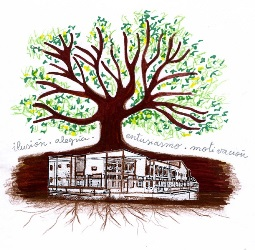
\includegraphics{../../img-Logos/iesoGalileo.jpg}} & Nombre y apellidos \hspace{120pt} & Ex. 3ºESO-D UD5:  & \\ 
        &&Ecuaciones& \\ 
        \hline
    \end{tabular}
    
    \begin{tabular}{| l | }
        \hline
        NOTAS: \\ 
            1. El examen tiene que ser limpio, ordenado y sin faltas de ortografía. \\
            
            2. El examen ha de realizarse en bolígrafo negro o azul, evitando tachones en la medida \\
            de lo posible. \\ 
            
            3. Deben aparecer todas las operaciones NO vale con indicar solo el resultado.\\
            
            4. Los problemas deben contener: Datos, planteamiento y resolución, respondiendo a lo \\
            que se pregunte, NO vale con indicar un número como solución del problema.\\

            5. Persona que se vea copiando o hablando con un compañero tiene un cero en el examen\\
            
        \hline
    \end{tabular}


    \begin{enumerate}

        \item Escribe la ecuación y resuelve: 
    
        (2 puntos) La quinta parte del cuadrado de un número es igual a la mitad de la suma de ese número y 5.
        $\vspace{5cm}$ 

        (1 punto) Dos veces el cuadrado de un número más ese número es igual a cero  $\vspace{7cm}$ 

        \item ( 1 punto) Resuelve la ecuación de primer grado
            \[(x-2)^2+(2-x)(x+3)=0\] $\vspace{5cm}$ 
        \item (1 punto)  Resuelve la ecuación de segundo grado
            \[(2x+4)(2x-4)=(x+3)^2+2(x+3)(x-3)\] $\vspace{5cm}$ 
        \item (1 punto) Resuelve la ecuación bicuadrada
            \[4x^4-5x^2+1=0\] $\vspace{5cm}$ 
                      
        \item (2 puntos) Reparte el número 20 en dos partes, de forma que la suma de sus cuadrados valga 202. $\vspace{5cm}$ 
        
        \item (2 puntos) La base de un rectángulo mide 4 cm más que la altura. Si disminuimos la altura en 1 cm, el área del nuevo rectángulo es de 84$cm^2$. $\vspace{5cm}$ 
    \end{enumerate}



\end{document}